\chapter{Validation} % possible chapter for Projects
\label{chap:validation}

This chapter describes the validation process of the framework. The validation process is divided into two parts: the validation of the framework
itself via unit and integration testing, and the validation of the framework's use cases via the demos.
Aspects of CI/CD used for the development and maintenance of the project will be explained, as well as the methodologies used to deploy the framework.
Finally, the~\Cref{sec:framework-limitations} describes the current limitations of the framework and future work geared toward extending and
improving the framework.

\section{Testing}
\label{sec:testing}

The \emph{software testing} is a method to check whether the actual software product matches the expected requirements and to ensure that the
software is ``defect free''. It involves the execution of software or system components using manual (not preferred) or automated tools to evaluate
one or more properties of interest. The goal of software testing is to identify errors, gaps or missing requirements in contrast to actual
requirements.

\subsection{Unit testing}
\label{sec:unit-testing}

\emph{Unit testing} is a type of software testing where the focus is on individual units or components of a software system.
Its purpose is to validate that each unit of the software works as intended meeting the requirements. Unit testing is usually performed by the
developer and is the first level of testing performed on the software.

Generally, unit tests are automated and executed whenever a change is made to the source code to ensure that the new code does not break the existing
functionality. Unit tests are designed to validate the smallest possible unit of code, such as a single function or method, testing them in
isolation from the rest of the system.

Usually, a lot of unit tests are written to try to cover as much code area as possible by going to test corner cases and wrong uses of the code.
One metric that indicates the amount of testing that is present in the code base is called code coverage.
This metric, often expressed as a percentage, defines how many lines of code were covered by unit tests (but not limited to) indicating the
pervasiveness of the tests. Attention should be paid to the fact that this metric is not an indication of good test quality but rather is intended to
be the opposite: this metric shows how many portions of the system are untested.
On the one hand, it might be counterintuitive, but by analyzing the concept of unit testing well, it is clear how it, too, is a part of software and
as such can be error-prone (thus not exhaustively testing the function or class) so it does not provide guarantees about the actual correctness of
the part of the code under test.
Nevertheless, unit tests are critical to intercepting most problems and avoiding the introduction of new ones.

The importance of testing has been recognized as a fundamental tool in the development and maintenance of a code base, and therefore
several test suites have been developed.
The most relevant in the JVM ecosystem are JUnit~\footnote{\textbf{JUnit} goal is to create an up-to-date foundation for developer-side testing on
	the JVM. \url{https://junit.org/junit5/}}
and TestNG~\footnote{\textbf{TestNG} is inspired by JUnit and NUnit but introduces some new functionalities that make it more powerful and easier to
	use. \url{https://testng.org/doc/}}, which are both unit-testing frameworks for the Java programming language.

In recent years, the concept has developed that tests themselves serve as specifications, and for that reason, they must follow good programming
practices (such as code) and be as clear and expressive as possible so that they can be easily read and interpreted.
In this regard, testing frameworks have emerged that provide DSLs enabling the writing of clear, well-organized and contextualized tests.
The most relevant in the JVM ecosystem are Spock~\footnote{\textbf{Spock} is a testing and specification framework for Java and Groovy applications.
	\url{http://spockframework.org/spock/docs/1.3/all\_in\_one.html}} and Kotest~\footnote{\textbf{Kotest} is a testing framework for Kotlin that
	provides a rich set of tools for testing. \url{https://kotest.io/docs/}}.

\paragraph*{}

The following will outline the unit testing aspects involved in the framework, explaining the rationale for choosing Kotest as the testing framework
and which key aspects of the framework were subject to unit testing.

The requirements that a testing framework must have for this project are as follows:
\begin{itemize}
	\item It must provide a DSL for writing tests
	\item It must provide several testing and assertion styles
	\item It must support out-of-the-box support for Kotlin coroutines
\end{itemize}

The first two requirements are needed to write clear and expressive tests, while the third is needed to test the framework in a seamless way since
is entirely based on coroutines.
The two main candidates for this project are Spock and Kotest. Although Spock provides a DSL for writing tests and different styles, it does not
provide any support for coroutine, since it was born for Java and groovy. In contrast, Kotest is entirely written in Kotlin and provides a full DSL
with various styles for testing, as well as native support for coroutines.
For these reasons, Kotest was chosen as the testing framework for this project. Moreover, Kotest supports Kotlin multiplatform, a feature that
perfectly fits the framework's goal of being cross-platform; in this way, all the tests are executed on the JVM, JS and Native platforms.

For most of the tests in the pulverization framework, the \emph{FreeSpec} style was used, which is a style that allows writing tests in a
specification-like way, where the test cases are written as a sentence, and the test body is written as a code block.
This style is particularly suitable for testing the framework since it allows writing tests clearly and expressively, the~\Cref{lst:free-spec} shows
an example of a test written in this style.

As can be seen, the test is written as a sentence in a specification-like fashion; in this way, even people who are not familiar with the framework
can understand the test and its purpose, as well as understand the framework API and its usage.

\lstinputlisting[
	language=Kotlin,
	label={lst:free-spec},
	caption={Example of a test written in the \emph{FreeSpec} style.}
]{listings/freespec-example.kt}

As follow will be described the relevant testing aspect for each module of the framework.

\subsubsection{Core module}

The core module is mainly composed of interfaces that the user must implement to use the framework. For this reason, the tests for this module
are limited and mainly focus on testing the \emph{configuration DSL} and the \emph{sensors container} and \emph{actuators container}.

The testing of the sensors and actuators container presents some interesting details that are worth mentioning.
The first aspect to consider is how the \emph{dependency injection} is performed during the tests. Is recalled that the \texttt{SensorsContainer} and
\texttt{ActuatorsContainer} implement the \texttt{PulverizedComponent} interface and therefore they must give an instance of the \texttt{Context}
interface. Although in this test scenario the context will not be used, it is necessary to provide an instance of the context to the container.
The fast and easy way to do this is to use a mocked version of the context, which is provided to the container via dependency injection.
The Koin framework makes available a \texttt{KoinTest} class and overriding the \texttt{getKoin} method, it is possible to provide a mocked version
of the context to the container. The \Cref{lst:mocked-context} shows an example of how to provide a mocked version of the context to the container.

\lstinputlisting[
	language=Kotlin,
	label={lst:mocked-context},
	caption={Example of how to provide a mocked version of the context to the container during the tests.}
]{listings/mocked-context.kt}

The effective test of the container is performed with the use of fixtures: the container to be tested requires some components like sensors, actuators
and so on to be added to it. For this reason, a fixture containing dummy components is created.
In this way, the test is focused on testing the container itself and not managing also the creation of the components, simplifying the overall test
class.

The test conducted on the container are trivial, but they are useful to ensure that the container is working properly.
the container is a delicate component in that it is queried through the type of the sensor or actuator to be retrieved, which is why it is necessary
to exhaustively test all possible scenarios that may occur. In particular, the functionality of sensors/actuators insertion was tested, but especially
the operations of retrieving instances of them, especially in the case of multiple instances of the same type of sensor/actuator are available in the
container.

\paragraph*{}

The testing of the DSL is also trivial: the DSL is a simple class that provides a set of functions to configure the framework. The tests are focused
on ensuring that the configuration produced is consistent with the use of the DSL.
In addition to testing in normal DSL use, special attention was paid to recreating possible uses of DSL that would lead to inconsistencies in
configuration and verify whether all such cases were handled correctly.
For example, was tested the case in which the user define the same component in two different deployment units, which is not allowed and should
produce an error. Finally, all the utility functions provided to work with the configuration were tested.

\subsubsection{Platform module}

The testing of the platform module is divided into four main parts: the testing of the \emph{communicator}, the testing of the
\emph{components reference}, and finally, the testing of the \emph{dsl}.

For what concern the \emph{communicator} testing, only the local communicator was tested, since the testing of the remote ones is delegated to the
specific module that implements them. The local communicator relies on the \texttt{CommManager} class to use the right flow for communication
with the other local communicator.
The test consists in registering the \texttt{CommManager} to the dependency injection module and then testing that the class returns
the same instance of the flow for the same communication type.

The testing of the local communicator, instead, is more complex.
First of all, is tested that the local communicator can not be initialized with a self-reference; that means that initialization of the local
communicator with the same component as source and destination is not allowed.
Then, is tested the communication between two local communicators: the test consists in creating two local communicators, spawning each one in a
different coroutine and then sending a message from one to the other. The test is successful if the message is received by the other local
communicator. If a problem occurs during the receiving of the message, the test can hang indefinitely, so a timeout is set to avoid this problem.
So the test fails if the timeout is reached or if the payload differs from sender to receiver, in all the other case the test succeed.
Finally, is tested the condition in which the sender sends more messages than the receiver can receive, in this case, the receiver should receive
only the last message sent by the sender. To emulate this condition, the sender and the receiver are spawned in different coroutines and the sender
starts sending messages to the receiver. The receiver, instead, when spawned is blocked for a certain amount of time, to emulate a slow receiver.
After the delay, the receiver starts collecting the messages sent by the sender but only the last one should be collected.

The testing of \emph{components reference} is straightforward: the test consists in creating a \texttt{ComponentsRefImpl} and then set up
it with the pair of the components to be referenced. After that, is tested that the reference is correctly set up and that the class
relies on the \texttt{LocalCommunicator} to send and receive the messages.

The \emph{dsl} testing is focused on testing possible illegal configurations of the platform. In this regard, several test cases were
created to test, for example, the case in which more or fewer components are registered than the one specified in the configuration.
During the development of a demo of the framework, it was discovered a bug in the DSL relative to the type inference; the bug was fixed and a test
was added to ensure that the bug will not be reintroduced in the future.

\subsubsection{Code coverage}

The code coverage represents an important indicator to be monitored during the development of a software project. In particular, the code coverage
of the project is managed by two different tools that operate at two different levels.
The first tool is \texttt{Kover}, which is a plugin for the \texttt{Gradle} build system that provides code coverage for Kotlin projects.
The second tool is \texttt{Codecov}, which is a service that provides code coverage for GitHub projects.

Kover operates at project-level: it instrument the test suite to collect the code coverage data and then it can publish code coverage report in
different formats, mainly \texttt{.html} and \texttt{.xml}.

On the other side, Codecov is a cloud service that collects the code coverage data from different sources and then provides a web interface
to visualize the code coverage of the project. All the coverage reports are uploaded to Codecov through the use of a \texttt{GitHub Action} that is
triggered every time a new commit is pushed to the repository. A more detailed description of the Codecov integration can be found in
the~\Cref{sec:ci-cd}.

\subsection{Integration testing}
\label{sec:integration-testing}

Integration testing is a type of testing that aims to test the interaction between different components of the system.
A typical software project is composed of several modules, and each one of them is responsible for a specific task; the integration testing
is focused on testing the interaction between these modules to ensure that they work together as expected when integrated.

There are four main approaches or strategies to perform integration testing: the \emph{bottom-up}, the \emph{top-down}, the \emph{big bang} and
the \emph{sandwich} approach. Each strategy has its own advantages and disadvantages, and the choice of the strategy to use depends on the
specific project and the type of testing that is required.

The \emph{big bang} approach involves integrating all modules at once and testing them all as one unit.
This approach has the following advantages:

\begin{itemize}
	\item It is easy to implement and it is suitable for small projects
	\item It is easy to identify errors, saving time and speeding up the deployment
\end{itemize}

However, the \emph{big bang} approach has the following disadvantages:

\begin{itemize}
	\item It is difficult to locate the source of the error since different modules are integrated as one unit
	\item It is time-consuming for large projects with lots of modules
	\item It must wait until all modules are developed before starting the testing phase
\end{itemize}

The \emph{top down} approach is an incremental approach that involves testing from the topmost module and then proceeding to the lower modules.
Each module is tested one by one and then integrated with the other modules. This approach has the following advantages:

\begin{itemize}
	\item It is easier to identify defects and isolate their sources
	\item Testers check important units first, so they are more likely to find critical design flaws.
	\item It is possible to create an early prototype of the system
\end{itemize}

The main disadvantage of the \emph{top down} approach is that when too many testing stubs are involved, the testing process can become complicated.

The \emph{bottom up} approach is the opposite of the \emph{top down} approach: it involves testing the lower modules first and then integrating
them with the upper modules. Once the lower-level modules are tested and integrated, then the next level of modules is formed.
The main advantages of using this approach are: easier to find and localize faults and no time is wasted waiting for all modules to be developed,
unlike the big bang approach. However, the main disadvantage of this approach is that critical modules which control the flow of the application are
tested last and may be prone to defects.

Finally, the \emph{sandwich} approach is a combination of the \emph{top down} and \emph{bottom up} approaches. In this approach, top down and bottom
up testing approaches are combined. The top-level modules are tested with low-level modules and the low-level modules are tested with high-level
modules simultaneously. Each module interface is tested, so there are fewer chances of a defect.
The main advantages derived from this approach are represented by the combination of the benefits of both top down and bottom up strategies.
Moreover, this approach reduces the amount of time spent on the process and all the modules are tested comprehensively.
The main disadvantage of this approach is that it is more complex than the other approaches.

\paragraph*{}

In the framework development, the \emph{big bang} approach was used to perform the integration testing. The reason for this choice is that
the framework is composed of a few modules, in this way a simpler integration testing process can be achieved.

The most important integration test is defined in the \texttt{AsyncScenario} test class. This test class is responsible for testing the
framework as a whole, in this test, are used the two DSLs to configure the devices and the platform, and then the platform is started testing
that each deployed component is correctly started and that the messages are correctly sent and received.
The importance of the test comes from the fact that it convolves the entire stack of the framework bringing all its components into play by verifying
that they are operating correctly.

\section{Continuous Integration and Delivery}
\label{sec:ci-cd}

The continuous integration and continuous delivery (CI/CD) pipeline is a set of automated processes that are used to build, test and deploy
the software. The main focus is on improving the software delivery throughout the software development lifecycle via automation.
Automating CI/CD throughout the software development lifecycle, including development, testing, production, and monitoring, allows organizations to
produce higher-quality code faster. While manual execution of CI/CD pipeline steps is possible, the real benefits come from automation.

The CI/CD pipeline is a systematic approach to software development that involves building, testing, and deploying code. Automating the pipeline
minimizes the risk of human error and ensures a consistent release process. It involves various tools, such as code compilation, unit testing, code
analysis, security, and binary creation.
CI/CD forms the foundation of a DevOps methodology and unifies developers and IT operations teams in software deployment.
The~\Cref{fig:ci-cd} shows a typical CI/CD pipeline.

\begin{figure}
	\centering
	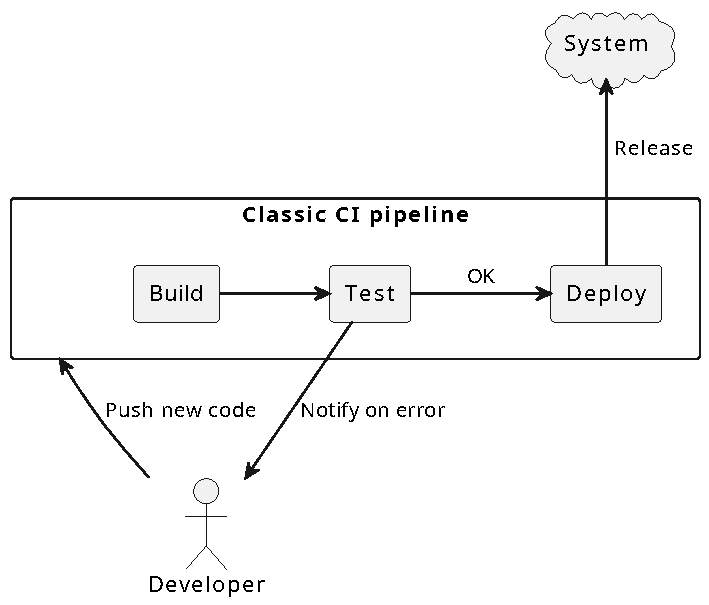
\includegraphics[width=0.9\textwidth]{figures/cicd-example.pdf}
	\caption{A classic example of a CI/CD pipeline.}
	\label{fig:ci-cd}
\end{figure}

To enable a pipeline, adequate tools and infrastructure are required. Over the last ten years, the CI/CD ecosystem has grown significantly,
and there are many tools available to support the pipeline.
As follow, a brief landscape of the most popular CI/CD tools is presented, showing the main features, the main advantages and disadvantages.

Jenkins is a free, open-source automation server that helps streamline the software development process by automating tasks such as building,
testing, and deploying code. It offers hundreds of plugins to support various technologies and tools, making it a highly versatile platform. Jenkins
is often used for continuous integration and continuous delivery (CI/CD) workflows, allowing developers to quickly and easily validate and release
code changes. A simple example of Jenkins use is to automate the building and testing of a Java application. The~\Cref{lst:jenkins-example} shows an example of a \emph{Jenkinsfile} written in Groovy syntax.

\lstinputlisting[
	language=Kotlin,
	caption={A Jenkinsfile example.},
	label={lst:jenkins-example}
]{listings/jenkins-example}

In the example, the Jenkinsfile defines a pipeline with two stages: one for building the application using Maven, and one for testing it. This is
just a simple example of what can be achieved with Jenkins, but it demonstrates how it can help automate and streamline the software development
process.

\emph{GitHub Actions} is a powerful CI/CD platform integrated into GitHub that allows developers to automate their software development workflows.
With GitHub Actions custom workflows that run on specific events can be defined, such as code pushes, pull requests, and releases. Workflows are
defined using \emph{YAML} files and can include multiple steps, such as building and testing code, deploying to various environments, and more.

Here is a simple example of a GitHub Actions workflow that builds and tests a Java application:

\lstinputlisting[
	caption={A GitHub Actions workflow example.},
	label={lst:github-actions-example}
]{listings/gha-example.yaml}

In this example, the workflow is triggered on pushes to the main branch and runs on an Ubuntu-based runner. The workflow includes steps to
check out the code, set up a Java environment, build the application, and run tests. With GitHub Actions, you can easily
automate and streamline your software development workflows, helping to improve efficiency and reduce errors.

An \emph{action} in the context of GitHub Actions is a pre-written, reusable piece of code that performs a specific task within a software development
workflow. These actions can be run as part of a workflow to automate tasks such as building code, testing it, deploying it, and more.

\paragraph*{}

The choice to use GitHub Actions to implement the CI/CD pipeline was made primarily for reasons of practicality and prior knowledge, but also because
it boasts a large community that supports and maintains the actions.
The pipeline is structured into three main jobs:

\begin{itemize}
	\item \textbf{Build}: the build job is responsible for running all the quality assurance tools, compiling the source code and generating the
	      artifacts
	\item \textbf{Test}: the test job runs all the unit tests and integration tests, and it is responsible to upload the artifacts on the
	      Maven Central repository and close the repository
	\item \textbf{Release}: the release job is responsible for releasing the artifacts on the Maven Central repository
\end{itemize}

All the aforementioned jobs are executed in parallel over three different operating systems: Windows, Linux and macOS.
The use of three different operating systems allows to verify that the framework is compatible with all the major operating systems and the relative
platforms, reducing the probability of errors on a specific platform.

When working with Kotlin multiplatform, the pipeline slightly changes, since the artifacts must be generated for each platform.
To achieve this, the pipeline is enriched with some additional jobs: the very first job is responsible for creating the staging repository on the
Maven Central repository, setting up the environment for a possible release. Then, are executed the build, test and release jobs for each platform.
A specific job is also added after the build job to close the staging repository on the Maven Central repository, and consequently, trigger the
checks over the repository. Finally, the release job is executed to release the artifacts on the Maven Central repository if needed.

\begin{figure}
	\centering
	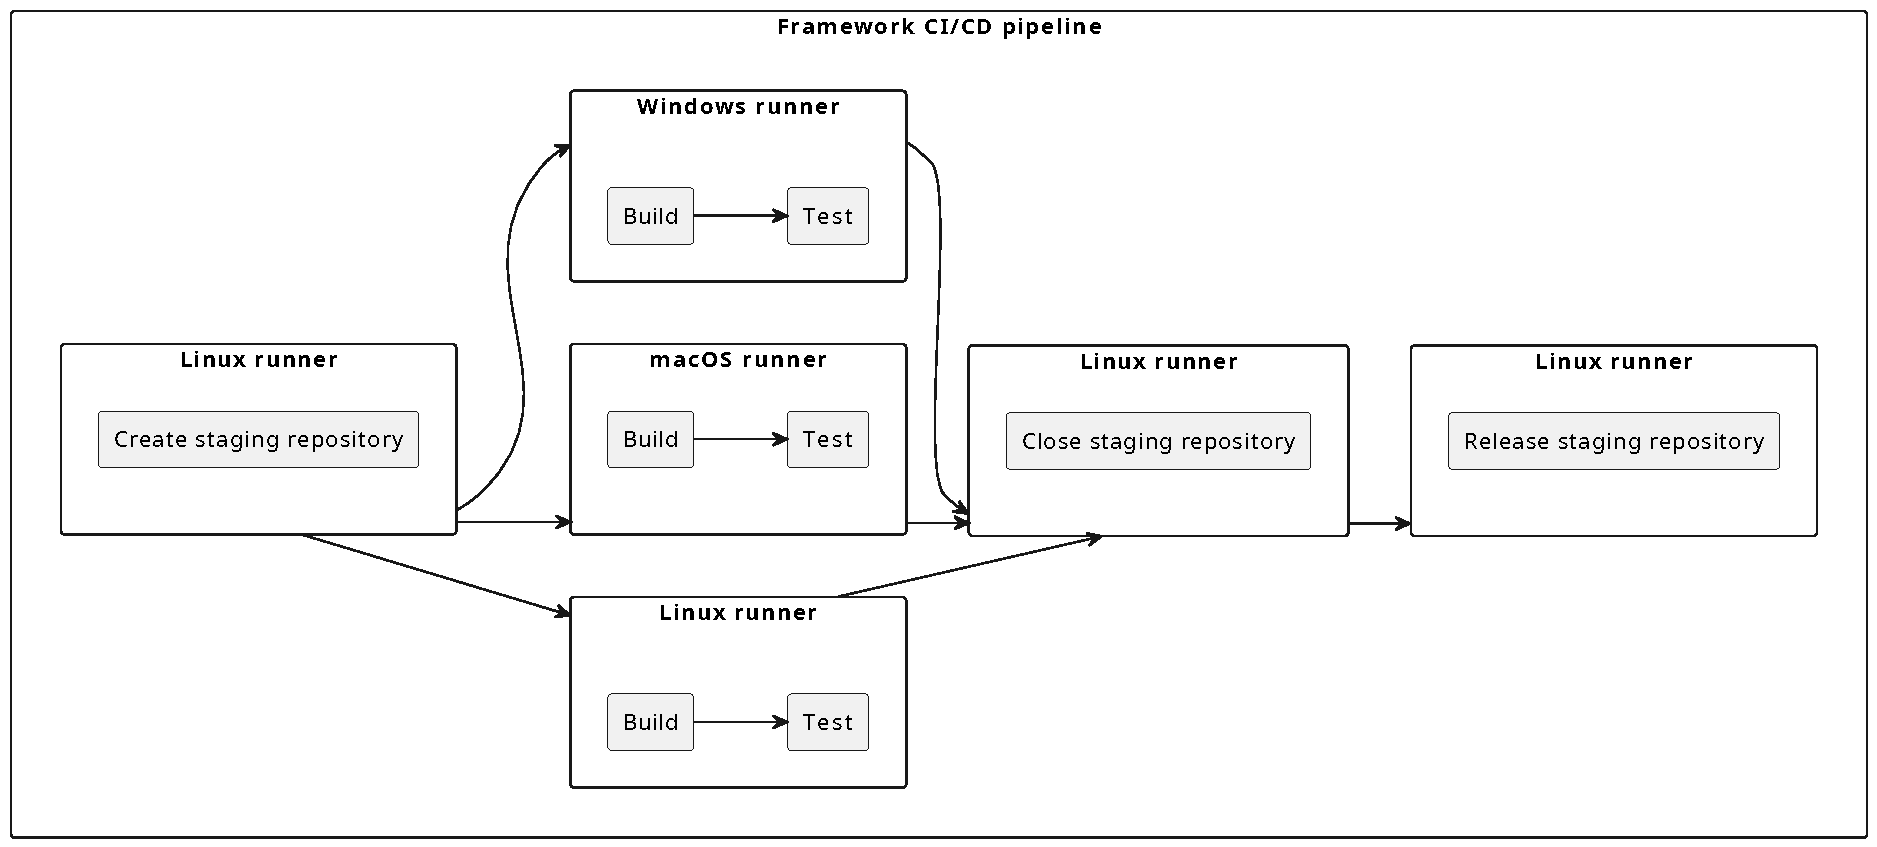
\includegraphics[width=\textwidth]{figures/framework-ci.pdf}
	\caption{The CI/CD pipeline of the framework.}
	\label{fig:ci-cd-pipeline}
\end{figure}

The rationale behind the choice of using a dedicated job for creating the staging repository is due the fact that the subsequent jobs are executed
in parallel over different OS, which means that they would create a staging repository for each OS, leading to an unintended condition.
Using the aforementioned approach, the staging repository is created only once, and then, the subsequent jobs are executed over the same repository
by sharing the \emph{repository id}. In this way, the artifacts coming from different OS are uploaded to the same repository (using the repository id
generated before), and consequently, the release job releases all the artifacts on the Maven Central repository consistently.

Code maintenance is a key aspect of good project lifecycle management.
For this reason, tools such as \emph{renovate} \emph{mergify} and \emph{semantic-release} have been used to automate these aspects.

Renovate is an automated tool that is used to manage and automate the process of updating
dependencies and keeping projects up-to-date. The Renovate Bot can be integrated into a project's code repository and configured to automatically
detect when updates are available and then create pull requests to implement the updates. This can help to streamline the process of keeping
dependencies up-to-date and reduce the risk of security vulnerabilities or compatibility issues.

Mergify is an automated tool that helps to manage and automate the process of merging pull requests in a code repository. The Mergify bot
can be integrated into a project's code repository and configured to automatically merge pull requests that meet specific criteria, such as passing
all required tests or receiving approval from a specified number of reviewers. This can help to speed up the code review process and reduce the
workload of maintainers, freeing them up to focus on more strategic tasks.

The semantic-release is a tool that automates the process of versioning and releasing software projects. It uses a specific commit message syntax to
determine the type of changes made in each commit~\cite{conventional-commits} and automatically generates a new version number and release based on
those changes.
This helps to ensure that version numbers are consistently and accurately updated, reducing the risk of errors and confusion, and allowing teams to
focus on more important tasks. Additionally, by automating the release process, semantic-release can help to speed up the development cycle and allow
teams to deliver new features and bug fixes to users more quickly and efficiently.

The joint use of these three tools on the one hand greatly speeds up the release and maintenance phases of the code but on the other hand, should be
paid attention to the fact that since are automatic tools, they could cause unintended updates causing repercussions on the proper functioning of the
project, such as updating a dependency that modifies a public API thus making it incompatible with its use in the code. To minimize these scenarios,
an extensive and complete test suite should be set up, but also a CI/CD pipeline that fails as soon as a problem is detected should be used; in this
way, maintainers are alerted and can proceed with manual intervention to resolve the issue.

Therefore, all these details have been carefully attended to so that no situations arise that lead to inconsistencies or
incompatibilities in the code base: renovate is configured to open a pull request as soon as a new version of any dependency is available; mergify is
configured to merge automatically the PRs coming from Renovate which the status check is passed, and semantic-release is configured to make a
release only from the \emph{master} branch and if the previous jobs are completed successfully.

\section{Demo 1: Single Device Multiple Components}
\label{sec:demo-1}

With the first demo, a simple system was aimed at highlighting the main aspects of pulverization instantiated in a real physical scenario.
As a second goal, the demo aims to provide a reference on how it is possible to ``pulverize'' a device through the framework by also testing it in a
context closer to real use cases.

This demo models the following scenario: you want to monitor the moisture status of soil through an able device
to sense the moisture in the soil and through a valve set the water flow to properly adjust the desired moisture level.
This simple scenario involves several aspects of the pulverization: first, we find the concepts of sensor and actuator, which respectively serve to
acquire the soil moisture level and regulate water flow. Finally, the behavior specifies how the flow regulation should occur against
the detected moisture. The~\Cref{fig:demo-1-system} shows the components defining the logical device.

\begin{figure}
	\centering
	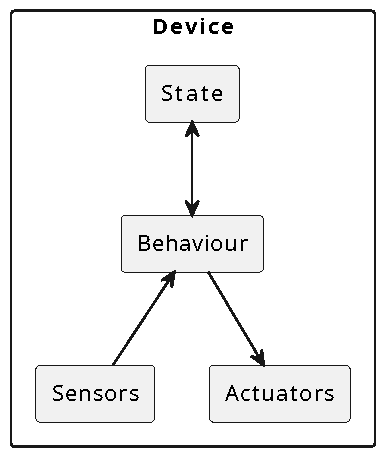
\includegraphics[width=0.4\textwidth]{figures/demo1-device.pdf}
	\caption{Decomposition of the moisture device into the pulverization components showing the interaction between them.}
	\label{fig:demo-1-system}
\end{figure}

The physical system is composed of three devices: two embedded systems used respectively for moisture sensing and water flow regulation and a server
which represents the infrastructure where the pulverized system runs.
Two \textbf{ESP32}~\footnote{\url{https://www.espressif.com/en/products/socs/esp32}} boards are used to implement the sensor component and the
actuator component. The main reason for choosing these boards is that they are cheap and easy to use. Moreover, they are equipped with a Wi-Fi
module, which allows them to communicate with the pulverization platform.

\begin{figure}
	\centering
	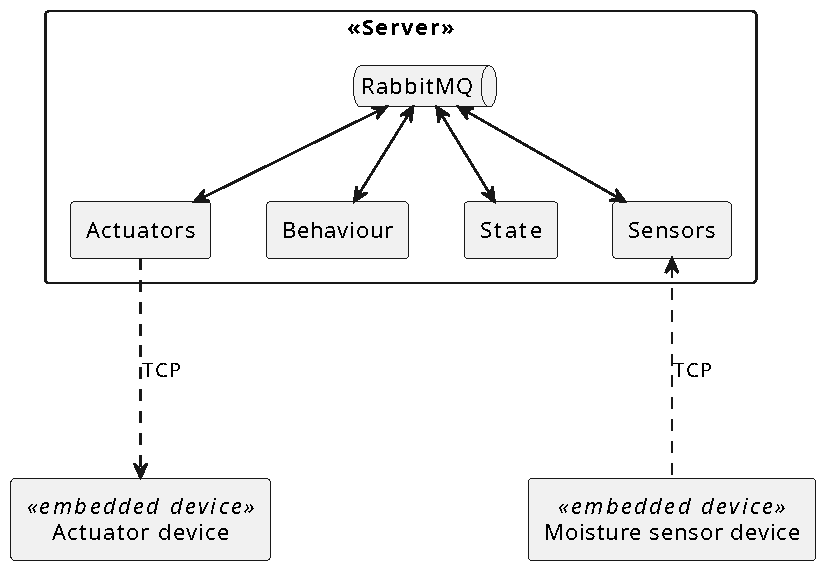
\includegraphics[width=0.7\textwidth]{figures/demo1-physical.pdf}
	\caption{Physical system architecture where are reported the communication between the components and the server.}
	\label{fig:demo-1-physical-system}
\end{figure}

In~\Cref{fig:demo-1-physical-system} is reported the physical system architecture where are reported the communication between the components and the
server.

The multiplatform nature of the framework allows the execution of each ``pulverized component'' on different architectures.
But at the time of writing, even if the number of supported architectures in Kotlin multiplatform is quite high, the framework does not support the
\textbf{Xtensa}~\footnote{\textbf{Xtensa} is a configurable and extensible processor architecture developed by Tensilica, now owned by Cadence Design
	Systems. It is designed to meet the unique requirements of a wide range of applications and systems, from low-power IoT devices to
	high-performance computing systems.}
architecture used by the ESP32 boards.

This limitation is solved directly by the framework: we can think of the \emph{sensor component} as acting as a kind of proxy by collecting data from
the embedded device. In this way, the firmware that will control the board will be written in a language that supports such architecture and will
provide a communication mechanism with the \emph{sensor component} that will simply forward the received message to other components.
As can be seen, the framework is extremely flexible, allowing it to accommodate limitations such as the one described above.

In this specific case, the limitation described above is solved by writing the \textbf{ESP32} firmware in \emph{Rust} (a language that supports the
Xtensa architecture) and implement the communication with the \emph{sensor component} using a TCP socket. The \emph{sensor component} is
implemented using the framework interface where a TCP socket is opened to listen for incoming messages from the embedded device.
On each received message, the sensor's value is extracted and saved in a local state; in this way, on each \texttt{sense} method call,
the last received value is returned.
This simple workaround allows the use of the pulverization framework also in devices that do not support the Kotlin multiplatform architecture.
The explanation of the limitation was made using the \emph{sensor component} as an example, but the same principle was applied to the
\emph{actuator component}, so again via TCP socket, a message is sent to the embedded device for opening or closing the valve.

As follow, are reported the main relevant details of the implementation of this demo.
As discussed above, the device has four components: \emph{sensor}, \emph{actuator}, \emph{behavior} and \emph{state};
the~\Cref{lst:demo-1-configuration} shows the configuration of the logical device where the \emph{sensor} and \emph{actuator} components are
deployed into two devices, and the \emph{behaviour} and \emph{state} components are deployed into the server.

\lstinputlisting[
	language=Kotlin,
	label={lst:demo-1-configuration},
	caption={Configuration of the logical device named ``moisture-device''.}
]{listings/demo-1-config.kt}

The \emph{behaviour} component defines the logic of the device: get the moisture level from the \emph{sensor} component and, if the moisture level
is below a threshold, open the valve using the \emph{actuator} component. The \emph{state} component is used to store the moisture level.
The~\Cref{lst:demo-1-behaviour} shows the implementation of the \emph{behaviour} component.

\lstinputlisting[
	language=Kotlin,
	label={lst:demo-1-behaviour},
	caption={Implementation of the \emph{behaviour} component for the demo 1.}
]{listings/demo-1-behaviour.kt}

Finally, the three deployment units are defined and containerized using Docker. In particular, a \emph{RabbitMQ} container is used to provide the
communication between the components, while the other three containers are used to run the \emph{sensor}, \emph{actuator} and \emph{behaviour}
components. Since the three components are deployed into three different containers, these may be deployed on different machines without affecting
the execution of the logical device.

The test of the demo was conducted on a local Linux machine running the four containers and the two ESP32 boards. All the containers are deployed
using \emph{Docker Compose}.
The two ESP32 boards are connected to the same Wi-Fi network and the \emph{sensor} and \emph{actuator} components are configured to connect to the
respective container using the IP address of the machine where the container is running.
Finally, the increase and decrease of soil moisture were simulated by verifying that the valve opened and closed properly.

\section{Demo 2: Multi Devices Multi Components}
\label{sec:demo-2}

Demo 2 aims to represent a more complex scenario than the previous one, involving multiple devices and enabling communication between them.
Also, we want to introduce more types of devices and show how they are supported by the framework.
This demo gets even closer to real scenarios involving multiple types of devices and where communication between them is a prerequisite.

This demo tries to replicate the hot-warm-cold game using two types of devices: an embedded device that needs to be found and many smartphones that
need to find it. The smartphones connect to the embedded device via Bluetooth, through which they determine its distance and communicate
this information with other smartphones. The embedded device receives the information on the distances of the smartphones and sets a light intensity
of an LED proportional to the proximity of the smartphones to it. Thus, the closer the smartphones are to the embedded device, the brighter the led
will emit; while the farther away the smartphones are, the less light will be emitted.
Each smartphone sends its distance to all other smartphones and simultaneously receives the distance of all other smartphones from the embedded
device. Sharing distance information is intended to test inter-device communication while simultaneously providing clues as to where the device that
needs to be found is located so that it can be found more quickly.

A Raspberry PI was used as the embedded device since it has both Wi-Fi and Bluetooth. The ESP32 was not chosen, as in the previous demo, because it
has hardware limitations that prevent Bluetooth and Wi-Fi from being used simultaneously. As for smartphones, Android smartphones were used, thus
allowing the framework to be tested on this platform as well.

When designing a pulverized system, it is good to represent the system from two different viewpoints: a viewpoint that captures the logical level
of the interactions between logical devices (see~\Cref{fig:demo-2-logical-diagram}) and a physical viewpoint that shows how the system is deployed in
the infrastructure (see~\Cref{fig:demo-2-physical-diagram}).

\Cref{fig:demo-2-logical-diagram} shows the network topology and how devices are tied together. This level of abstraction is what should be used by
the user who intends to implement the system by exploiting the pulverization framework: he or she does not have to worry about infrastructure or
deployment aspects; how communications take place is handled directly by the framework. This greatly simplifies the development of the system. How
then the system is deployed in the infrastructure is depicted in~\Cref{fig:demo-2-physical-diagram}, which shows at the physical level where
components are run and how intra-component communications of each device take place, also, are depicted all the physical devices involved in the
system.

\begin{figure}
	\centering
	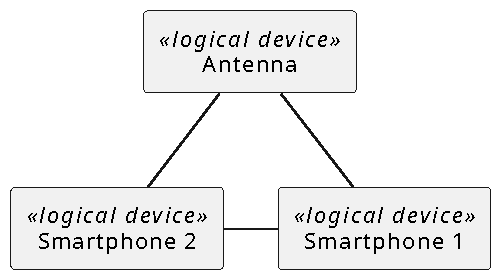
\includegraphics[width=0.6\textwidth]{figures/demo2-logical-device.pdf}
	\caption{Logical diagram of the connection between the logical devices.}
	\label{fig:demo-2-logical-diagram}
\end{figure}

\begin{figure}
	\centering
	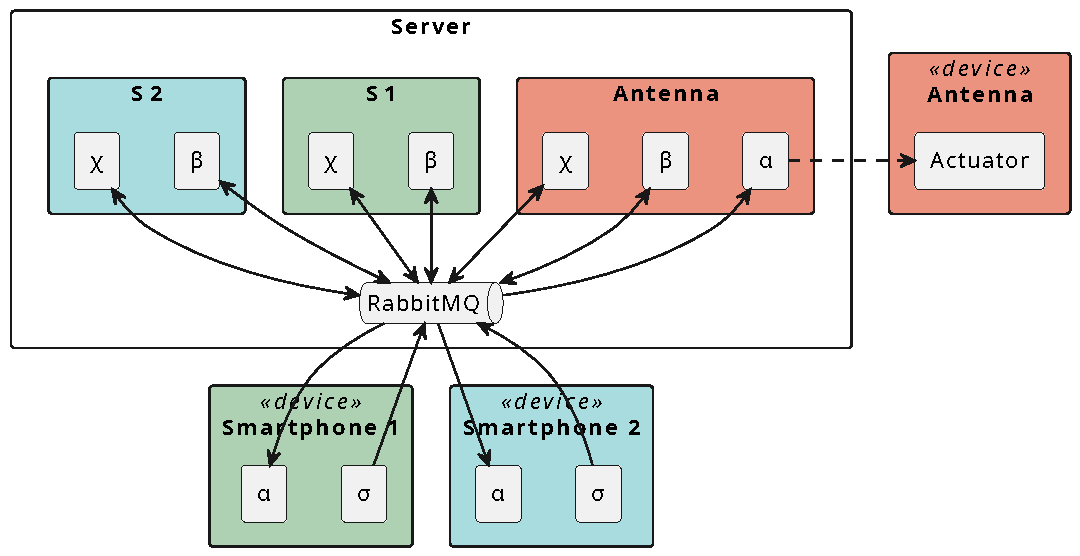
\includegraphics[width=\textwidth]{figures/demo2-physical.pdf}
	\caption{Physical diagram of the connection between the logical devices.}
	\label{fig:demo-2-physical-diagram}
\end{figure}

Design choices for the implementation of the demo are explained below. The demo is divided into four main modules:

\begin{itemize}
	\item \textbf{Android application:} in this module is implemented the mobile application that runs on smartphones
	\item \textbf{Raspberry PI firmware:} this module implements the firmware that runs on the Raspberry PI
	\item \textbf{Common module:} this module contains the common code shared between the \emph{Platform} and \emph{Android application} modules
	\item \textbf{Platform module:} this module contains the code that runs all the devices' components logics.
\end{itemize}

The \emph{common module} contains the code shared between the \emph{platform} and \emph{android application} modules. In particular, it contains
the implementation of each component like the \emph{behaviour, sensors} and \emph{actuators} components, either for the embedded device and the
smartphones. The reason why all the components are implemented in the same module is that they can be reused whenever a new device is added to the
system. In this way, the specific device should not implement its specific version of the component but instead reuse the one already implemented.

The android application is structured as follows: during the \emph{initialization} stage the pulverization platform with its components is
initialized and the \emph{Bluetooth LE} module configured. Then, a user interface is shown to the user, which allows them to start the system by
providing the IP of the machine where the platform is running and the device id. Once the user starts the system, the \emph{Bluetooth LE} module
starts scanning for nearby devices and, when the embedded device is found (the Raspberry PI), the \emph{Bluetooth LE} module connects to it and
starts sending the distance information to all its neighbours. At the same time, the application listen for incoming messages from the neighbours
and shows their distance on the screen.

The Raspberry PI firmware is structured as follows: first of all, the \emph{Bluetooth LE} module is configured as a server and starts the
advertising process, so that all the nearby devices can connect to it. Then, a TCP socket is opened toward the \emph{actuator component} deployed
on the server. Once the connection is established, all the incoming messages are collected. The message contains a decimal value between $0$ and $1$
that respectively means LED turned off and LED turned on; all the intermediate values are used to set the LED intensity.

Finally, the \emph{Platform} module defines for each logical device in the system all its deployment units. In particular, runs the
\emph{behaviour, sensors} and \emph{actuators} components for each smartphone and the \emph{behaviour} and \emph{actuators} components for the
embedded device.

The system was dockerized and deployed using docker compose. The system, once started, was tested by making use of two smartphones that were
continuously moved around the room to observe how it varied the LED intensity accordingly. The test conducted did not reveal any anomalies or
malfunctions, except for some inaccuracies in the calculation of the distance of the devices from the Bluetooth antenna due to signal
fluctuations.

One notable test that has been conducted involves simulating a device failure and observing how the system reacts to this condition.
The failure of a device was simulated by disconnecting it from the network.
As soon as the device was disconnected from the network, the system continued to function as expected. Devices that were still active, store the last
message received from that device and thus did not alter their behavior. When the device returns operational in the network, then it will start
sending the newly updated data to its neighbors again, which will then update the information about that device's distance from the antenna.

In conclusion, this demo brought out the effectiveness of the framework in clearly separating business logic development from infrastructural and
deployment aspects, highlighting how more complicated systems are achievable through the sprinkling framework. Again, it highlighted how a failure of
one component of the system does not preclude its operation in its entirety.

This demo can be extended by going to improve the calculation of the distance of the devices from the antenna, for example, by implementing a filter
that reduces the noise in the signal acquisition producing more stable and truthful values. Another interesting aspect to analyze may be to have some
smartphones with all components running on them, while other smartphones have the behavior running in the cloud, thus observing that the overall
behavior does not change as the deployment structure changes.

\section{Demo 3: crowd estimation}
\label{sec:demo-3}

\todo{Valutare se questa demo è da inserire dal momento che non c'e' stato tempo di realizzarla}

\section{Current framework limitations}
\label{sec:framework-limitations}

At present, the framework partially implements the concept of pulverization: dynamics and support for different protocols are some examples of
shortcomings.
The goal of this section is therefore to provide an overview of the main shortcomings of the framework by going on to examine in what contexts these,
if implemented, could solve certain problems.

\subsection{Dynamics}
\label{sec:dynamics}

By dynamism in this context we mean the ability of the framework to be able, dynamically, to relocate pulverized components in the infrastructure.

At present, the framework does not handle this aspect: the deployment structure is defined a priori and remains so throughout the life of the
executed system. Although dynamism is a key aspect in pulverization, it was decided to focus more on good domain modeling to build a solid foundation
on which the framework can be extended, rather than implementing as many aspects as possible running the risk of creating a rigid framework that is
not very extensible and difficult to use.

\subsection{Multi-protocols}
\label{sec:multi-protocols}

The management of multiple protocols to enable intra-component communication is an important aspect since sputtering can involve a large number of devices that are also heterogeneous with each other and therefore have different computational and even communication capabilities.

For this reason, the choice of one protocol over another is not mutually exclusive, but it may be appropriate, for example, to provide
multiple protocols that are used in the pulverized system. Again, you might be dealing with devices that do not support certain protocols, or you are
in a situation where you want to use a very lightweight protocol (e.g. MQTT) for devices with very low computational resources and instead use a
higher-performance protocol for those parts of the system with high computational power on board.

At the time of writing, the only protocol implemented to enable intra-component communication is RabbitMQ as it represents a good compromise between
ease of use, performance and adoption.

Adoption of additional protocols would increase the framework's potential to be used in many contexts with strong device heterogeneity.